\section{Experimental results and analysis}
\label{sec:results}

\subsection{Answer to RQ1: contract reliability}
\label{sec:exp-safety}

\begin{table}
\caption{RQ1: probability (over 1000 calibration draws) that the
deployed policy's \emph{exact risk on the full finite population}
exceeds $\alpha$ --- the quantity the certificate actually bounds ---
and mean cost relative to always running the strongest plan. Cells
where no violating draw was observed report the one-sided 95\%
binomial upper bound $<.003$ rather than an absolute rate: each
policy's population risk is one exact number, so draws vary only
through \emph{selection}, and $<.003$ means no draw selected an
out-of-contract policy. \system\
is the only method meeting the $\delta=0.1$ budget on all benchmarks.}
\label{tab:safety}
\centering
\setlength{\tabcolsep}{1.7pt}\scriptsize
\begin{tabular*}{\tblwidth}{@{}lcccccccc@{}}
\toprule
& \multicolumn{2}{c}{HybridQA} &
\multicolumn{2}{c}{CRAG} &
\multicolumn{2}{c}{ASQA} &
\multicolumn{2}{c}{QAMPARI} \\
& \multicolumn{2}{c}{($\alpha{=}.35$)} &
\multicolumn{2}{c}{($\alpha{=}.65$)} &
\multicolumn{2}{c}{($\alpha{=}.25$)} &
\multicolumn{2}{c}{($\alpha{=}.66$)} \\
Method & viol. & cost & viol. & cost & viol. & cost & viol. & cost \\
\midrule
Empirical (no cert.) & .470 & .19 & .493 & .15 & .408 & .45 & .451 & .45 \\
BO-tuned             & .572 & .12 & .005 & .08 & .410 & .12 & .532 & .21 \\
Utility router       & .160 & .07 & $<$.003 & .03 & .106 & .08 & .497 & .40 \\
Abacus               & .099 & .34 & .275 & .16 & $<$.003 & .25 & .433 & .51 \\
\system\ (ladder)    & .006 & .31 & .005 & .38 & .002 & .51 & .004 & .75 \\
\system\ (full)      & \textbf{$<$.003} & .11 & \textbf{$<$.003} & .07 & \textbf{$<$.003} & .43 & \textbf{.001} & .84 \\
\bottomrule
\end{tabular*}
\end{table}

\begin{figure}
\centering

\includegraphics[width=\columnwidth]{figures/violation_sweep.pdf}
\caption{RQ1: probability that the deployed policy's exact
finite-population risk exceeds $\alpha$, across 1000 calibration draws
as the contract level varies (thirteen settings across four
benchmarks). The dotted line is the certified budget $\delta=0.1$;
only \system\ stays below it everywhere.}
\label{fig:sweep}
\end{figure}

\begin{figure}
\centering

\includegraphics[width=0.72\columnwidth]{figures/calibration.pdf}
\caption{RQ1: target level $\alpha$ versus realized violation of the
certified policy (test split). All points lie on or below the diagonal
up to test-sampling noise: valid but tight.}
\label{fig:calibration}
\end{figure}

Table~\ref{tab:safety} reports the repeated-draw protocol of
Section~\ref{sec:protocol}: violation here means the selected policy's
\emph{exact} risk on the full finite population exceeds $\alpha$, so
Table~\ref{tab:safety} verifies the theoretical claim directly, with
no test-sampling noise in the verdict; Figure~\ref{fig:sweep} sweeps
the contract level across thirteen settings on the same
population-risk criterion. Three observations emerge. First,
empirically tuned methods select policies whose \emph{true} risk is
out of contract in 41--57\% of draws on their worst benchmark ---
these are genuine failures of the deployed policy, not artifacts of a
noisy test split; across the full sweep no baseline stays below
$\delta$ everywhere. Second, the certified methods hold the
population-level promise with margin: the full optimizer's true risk
exceeds $\alpha$ in at most 0.1\% of draws at the headline levels ---
below $.003$ on HybridQA, CRAG, and ASQA, a single violating draw on
QAMPARI, and never above
0.8\% anywhere on the sweep --- an order of magnitude
inside the $\delta = 10\%$ budget. Rates this small are the
\emph{predicted} outcome, not an artifact: the test certifies only
candidates whose calibration risk clears $\alpha$ by the
finite-sample radius ($0.02$--$0.07$ at these $n$), so deploying an
out-of-contract policy requires a false certification whose realized
probability is far below its $\delta$ bound; where the 1000 draws
contain no such event we accordingly report the binomial upper bound
$<.003$, the resolution limit of the protocol, rather than an
absolute rate. The same quantization explains the
occasional near-floor baseline entries --- e.g., the utility router at
CRAG's loose $\alpha = .65$ selects only policies whose fixed
population risk happens to sit below the threshold (below the
protocol's resolution here, yet
22.1\% on the noisier held-out criterion, and far above $\delta$ at
other levels in Figure~\ref{fig:sweep}) --- a coincidence of one
setting, not a guarantee. On the
conventional held-out criterion the certified policies show 0--7\%
rates:
the difference between the two criteria is pure test-split binomial
noise, which the population protocol removes.
Figure~\ref{fig:calibration} shows the certificates are tight rather
than vacuous: where the contract binds, realized risk tracks $\alpha$
with a margin of 0.02--0.07 that shrinks with calibration size, exactly
the finite-sample radius of the underlying test. Third, safety is not
purchased with money: on CRAG the full optimizer is both the safest and
among the cheapest, because the richer certified family (jump routers)
dominates threshold tuning. Abacus is safe exactly when inter-plan gaps
are large relative to its sampling noise (ASQA) and unsafe when they
are not (CRAG, 28\%; QAMPARI, 43\%) --- point estimates cannot tell
these regimes apart, which is the core argument for certification.

\paragraph{Slice-level reliability}
Marginal risk control can hide systematic failures on identifiable
slices. On CRAG, with group-wise contract levels
$\alpha_{\mathrm{static}} = .62$, $\alpha_{\mathrm{slow}} = .72$,
$\alpha_{\mathrm{fast}} = .92$, and $\alpha_{\mathrm{rt}} = .93$, a
single marginally certified policy violates the real-time group's
contract in 99\% of 200 draws (realized risk 0.99 against a 0.93
target: the cheap rungs it certifies for the average workload have no
fresh evidence for real-time queries). Group-conditional certification
(Section~\ref{sec:families}) brings every group to at most 3.5\%,
escalating real-time queries to the knowledge-graph-API rung while
\emph{lowering} static-group cost. When a group's contract is
infeasible in the plan space --- fast-changing queries at
$\alpha = .65$, where even the strongest plan's group risk is 0.79 ---
\system\ reports non-certifiability instead of silently
under-delivering.

\smallskip\noindent\textbf{Answer to RQ1:} \emph{verified directly on
exact finite-population risk, point-estimate feasibility is a coin
flip --- uncertified tuners deploy truly out-of-contract policies in
up to 64\% of draws --- whereas certification keeps the
$\delta$-promise with an order of magnitude to spare at every contract
level tested, extends it to query slices, and reports infeasibility
honestly.}

\subsection{Answer to RQ2: cost-efficiency at matched contracts}
\label{sec:exp-cost}

\begin{table}
\caption{RQ2: single-draw test-split empirical risk / mean cost (mCNY
per query) at representative contract levels. Bold: the certified
policy. A certified policy's \emph{population} risk satisfies the
contract with probability $\ge 1-\delta$ (verified in
Table~\ref{tab:safety}); its test-split entry here carries binomial
noise of $\pm .01$--$.04$ and may sit on either side of $\alpha$.
The matched oracle is the cheapest hindsight per-query assignment with
test mean loss $\le \alpha$ (same objective as \system); the zero-loss
skyline solves a stricter objective and is not cost-comparable.}
\label{tab:main}
\centering
\setlength{\tabcolsep}{2.2pt}\scriptsize
\begin{tabular*}{\tblwidth}{@{}lcccccccc@{}}
\toprule
& \multicolumn{2}{c}{HybridQA} &
\multicolumn{2}{c}{CRAG} &
\multicolumn{2}{c}{ASQA} &
\multicolumn{2}{c}{QAMPARI} \\
& \multicolumn{2}{c}{$\alpha{=}.34$} &
\multicolumn{2}{c}{$\alpha{=}.65$} &
\multicolumn{2}{c}{$\alpha{=}.216$} &
\multicolumn{2}{c}{$\alpha{=}.71$} \\
Method & risk & cost & risk & cost & risk & cost & risk & cost \\
\midrule
Fixed strongest      & .290 & 7.21 & .600 & 6.00 & .116 & 9.01 & .610 & 6.49 \\
Complexity router    & .509 & 1.46 & .620 & 4.74 & .281 & 1.14 & .612 & 6.47 \\
Utility router       & .387 & 0.40 & .625 & 0.28 & .223 & 1.02 & .712 & 0.43 \\
BO-tuned             & .380 & 0.97 & .621 & 0.89 & .221 & 1.41 & .708 & 0.94 \\
Abacus               & .321 & 1.75 & .600 & 6.00 & .201 & 1.31 & .666 & 1.23 \\
Empirical (no cert.) & .372 & 1.45 & .635 & 1.39 & .199 & 5.67 & .784 & 1.84 \\
\system\ (ladder)    & .358 & 2.11 & .618 & 2.16 & .165 & 6.42 & .724 & 2.88 \\
\system\ (full)      & \textbf{.338} & \textbf{1.05} & \textbf{.624} & \textbf{0.30} & \textbf{.145} & \textbf{6.56} & \textbf{.712} & \textbf{0.43} \\
\midrule
Matched oracle       & .340 & 0.33 & .649 & 0.18 & .214 & 0.98 & .710 & 0.30 \\
Zero-loss skyline    & .193 & 2.97 & .491 & 4.74 & .056 & 2.83 & .514 & 5.47 \\
\bottomrule
\end{tabular*}
\end{table}

\begin{figure}
\centering

\includegraphics[width=0.86\columnwidth]{figures/cost_risk_hybridqa.pdf}
\caption{RQ2: cost--risk positions on HybridQA at $\alpha=0.34$ (test
split). Certified methods sit below the contract line; uncertified
tuners that are cheaper sit above it.}
\label{fig:tradeoff}
\end{figure}

Table~\ref{tab:main} and Figure~\ref{fig:tradeoff} fix representative
contract levels and show one draw each; the guarantee behind the bold
rows is the population-level one verified in Table~\ref{tab:safety}.
At $\alpha = 0.34$ on HybridQA, \system\ certifies a jump-router
policy costing 1.05 mCNY per query with test risk 0.338 ---
6.9$\times$ cheaper than the strongest plan (7.21 mCNY, risk 0.290);
the uncertified methods that undercut it do so by breaking the
contract (utility router: risk 0.387 $> \alpha$ at 0.40 mCNY). At
$\alpha = 0.65$ on CRAG, the certified policy costs 0.30 versus 6.00
mCNY (20$\times$); at $\alpha = 0.71$ on QAMPARI, 0.43 versus 6.49 mCNY
(15$\times$) --- here certification adopts the utility router's own
policy, showing that the certified family subsumes the baselines'
policies and differs only in the feasibility test. On ASQA
($\alpha = 0.216$), the certified policy's test risk is 0.145 at 6.56
versus 9.01 mCNY, while the utility router (0.223) and BO (0.221) sit
above $\alpha$. Several single-draw entries of certified ladder
policies sit slightly above $\alpha$ (e.g., 0.358 vs.\ 0.34 on
HybridQA, 0.724 vs.\ 0.71 on QAMPARI): these are within one standard
error of test-split noise, and the repeated-draw protocol of
Table~\ref{tab:safety} confirms the corresponding population risks
violate in at most 0.6\% of draws --- what certification promises is
the distributional guarantee, not that every finite sample lands below
$\alpha$. The fair skyline for \system's objective is the
\emph{matched oracle} --- the cheapest hindsight per-query assignment
with test mean loss $\le \alpha$, unattainable since it requires
knowing each answer's outcome in advance. \system\ pays
1.4--3.2$\times$ its cost on HybridQA, CRAG, and QAMPARI, and
6.7$\times$ on ASQA, where two-constraint feasibility forces a more
conservative policy; the gap is the price of feasibility established
from finite samples rather than hindsight. The zero-loss skyline row
solves a different, stricter problem (no loss on any query) and is
reported only for context --- comparing contract-feasible costs
against it is not meaningful, and on three of four benchmarks \system\
is in fact cheaper than it. When the contract is infeasible for every
candidate, \system\ correctly refuses to certify and falls back to
best effort.

\paragraph{Strict contracts via certified deferral}
The headline levels above are dictated by what today's pipelines can
achieve while answering everything; a regulated deployment wants
$\alpha \le 0.2$. With the D-family (Section~\ref{sec:families}),
\system\ certifies the pair $\Prob(\text{answered} \wedge
\text{violating}) \le \alpha$, $\Prob(\text{deferred}) \le \beta$. At
$\alpha = 0.1$ it certifies HybridQA at deferral budget $\beta = 0.75$
(test: answered-and-violating 0.091, deferral 0.597) and ASQA at the
same budget with far less deferral used (0.087, 0.219; cost 7.64 vs.\
10.90 mCNY for the strongest plan); at $\alpha = 0.2$ all four
benchmarks certify --- ASQA defers only 2.9\% of queries at
$\beta = 0.25$, CRAG needs $\beta = 0.75$ (deferral 0.529), QAMPARI
0.678 --- and at $\alpha = 0.05$ no benchmark certifies at any tested
$\beta \le 0.9$, which \system\ reports as infeasible rather than
shipping a policy that cannot keep the promise. Strictness is thus
purchased transparently with deferral volume, and the human-review
load is itself certified, not discovered in production.

\paragraph{Joint multi-dimensional contracts}
Production contracts bind several dimensions at once. On CRAG we
certify a four-constraint contract --- correctness $\le .65$,
hallucination $\le .30$, staleness $\le .05$, latency-budget
exceedance $\le .10$ (8 s) --- via the intersection--union test:
the certified policy satisfies all four on test (correctness .603,
hallucination .258, latency .057, all p-values
$\le 5.5\times 10^{-3}$) at 5.02
mCNY per query; the staleness loss never fires on the 1006-query test
split ($<.003$ at 95\% confidence) because the certified policy
escalates every stale-evidence query. IUT certifies 47 candidates against Bonferroni's 44
and selects a 3\% cheaper policy --- testing each constraint at full
level $\delta$ instead of $\delta/4$ is uniformly more powerful. On
ASQA (citation recall $\le .25$, citation precision $\le .35$, quality
$\le .40$, latency $\le .15$ at 15 s) the gap is qualitative:
IUT certifies 45 candidates (test risks $.188/.230/.261/.033$) while
Bonferroni certifies \emph{none} --- at $n_{\mathrm{cal}} = 350$ the
$\delta/4$ correction is fatal, exactly the failure mode
Section~\ref{sec:certification} predicts.

\smallskip\noindent\textbf{Answer to RQ2:} \emph{the guarantee costs
little --- the certified policy is 6.9--20$\times$ cheaper than the
strongest fixed pipeline and within 1.4--6.7$\times$ of the matched
hindsight oracle; strict contracts down to $\alpha = 0.1$ certify once
deferral is priced in, four-constraint joint contracts certify with
IUT where Bonferroni fails, and every method that beats \system\ on
cost does so by breaking the contract.}

\subsection{Answer to RQ3: risk vouchers and composition}
\label{sec:exp-rewrites}

\begin{table}
\caption{RQ3: rewrite vouchers on HybridQA
($n_{\mathrm{cal}} = 500$; cost in mCNY per query). Harm $=$ loss
strictly worse than the base
plan's. A voucher is a $1-\delta_r$ confidence bound, so its
guarantee is \emph{coverage over repeated calibration draws}, not
dominance of any single test sample: over 1000 draws against the exact
harm rate of the pooled 1000-query population, every voucher covers in
$\ge 98.9\%$ of draws against a $95\%$ nominal level (right column).
The three composition rows price the \emph{same} composed plan, so
their execution columns (cost, harm) coincide by construction; the
rows differ only in how the bound is built. The telescoping voucher
covered in every one of the 1000 redraws, reported as the one-sided
95\% lower bound $>$.997 against its nominal
level of $.80$ ($m = 4$ steps at $\delta_r = .05$) --- the deliberate
price of dropping the no-synergistic-harm (NSH)
assumption, which this workload violates (8\% synergistic harm); the
telescoping path voucher (Proposition~\ref{prop:composition}) is
assumption-free at 10\% extra width over the (invalid) union bound.}
\label{tab:rewrites}
\centering
\setlength{\tabcolsep}{1.5pt}\scriptsize
\begin{tabular*}{\tblwidth}{@{}l@{\extracolsep{\fill}}cccccc@{}}
\toprule
Variant & cost & harm$_{\mathrm{cal}}$ & voucher $\hat\eps$
& harm$_{\mathrm{te}}$ & harm$_{\mathrm{pop}}$ & cover. \\
\midrule
base $P^\ast$    & 1.74 & ---  & ---  & ---  & --- & --- \\
R1 prefilter     & 1.75 & .014 & .026 & .030 & .022 & .995 \\
R2 $k$-trunc     & 1.11 & .060 & .081 & .084 & .072 & .991 \\
R3 no-rerank     & 1.69 & .058 & .078 & .070 & .064 & .994 \\
R4 gen-downgr.   & 0.33 & .130 & .157 & .152 & .141 & .989 \\
\midrule
comp.\ (union, NSH)   & 0.21 & .218 & .342 & .262 & .240 & --- \\
comp.\ (telescoping)  & 0.21 & .218 & .376 & .262 & .240 & $>$.997 \\
comp.\ (direct cert.) & 0.21 & .218 & .251 & .262 & .240 & .989 \\
\bottomrule
\end{tabular*}
\end{table}

On HybridQA we fix a base plan (hybrid retrieval $k = 16$, rerank,
plus-tier generator), apply four single rewrites, all chain prefixes,
and the full composition on 500 calibration and 500 test queries
(Table~\ref{tab:rewrites}). A voucher is a confidence bound, so the
correct empirical test is its coverage: pooling calibration and test
into a fixed 1000-query population and redrawing the 500-query
calibration set 1000 times, each single-rewrite voucher covers the
population's exact harm rate in 98.9--99.5\% of draws --- above its
95\% nominal level (Clopper--Pearson, $\delta_r = .05$), as the
one-sided bound's conservatism predicts. (A single test-split column
can land on either side of the voucher, as R1 and R2 do in the table;
that is binomial noise, not a coverage failure.) The harm ordering ---
prefilter $<$ rerank-elision $\approx$ $k$-truncation $<$ generator
downgrade --- matches the intuition that evidence-preserving rewrites
are safest. The composed plan cuts cost 8.3$\times$ (1.74 to 0.21
mCNY) with population harm 0.240.

\paragraph{Composition}
The base-relative union bound (0.342) requires the no-synergistic-harm
assumption --- and the data \emph{violate} it: 8\% of harmed queries
are harmed only by the composition (synergy between truncation and
generator downgrade), so that bound's nominal coverage is unfounded
even where its number happens to be large enough. The telescoping path
voucher of Proposition~\ref{prop:composition} (step vouchers
$.026/.081/.105/.164$, sum 0.376) costs only 10\% extra width over the
union bound while being assumption-free --- and it covered the
population chain harm in every one of the 1000 redraws ($>$99.7\% at
95\% confidence). Both remain looser
than the direct certificate (0.251 mean, 98.9\% coverage) on the
deployed chain --- which is why \system\ uses vouchers to order search
and certifies directly.

\paragraph{Selectivity conditioning}
The flat prefilter voucher ($\hat\eps = .026$) is marginally valid but
hides heterogeneity that the planner's selectivity estimate exposes:
stratifying by pool selectivity $\sigma$, realized test harm is 0.075
on the vague-predicate stratum --- three times the flat voucher ---
versus none observed on the fully selective stratum. The per-stratum vouchers
($.076/.088/.128/.020$) cover every stratum's realized harm, giving the
rewrite search a risk signal that tracks \emph{which} queries a
pushdown endangers rather than an average.

\smallskip\noindent\textbf{Answer to RQ3:} \emph{vouchers achieve at
least 98.9\% repeated-draw coverage against their 95\% nominal level
and are correctly ordered; assumption-free telescoping composition
costs only 10\% width over a union bound whose assumption the data
falsify; selectivity conditioning turns a marginal voucher into a
per-stratum risk signal.}

\subsection{Answer to RQ4: knowledge drift detection and recovery}
\label{sec:exp-drift}

\begin{figure*}
\centering
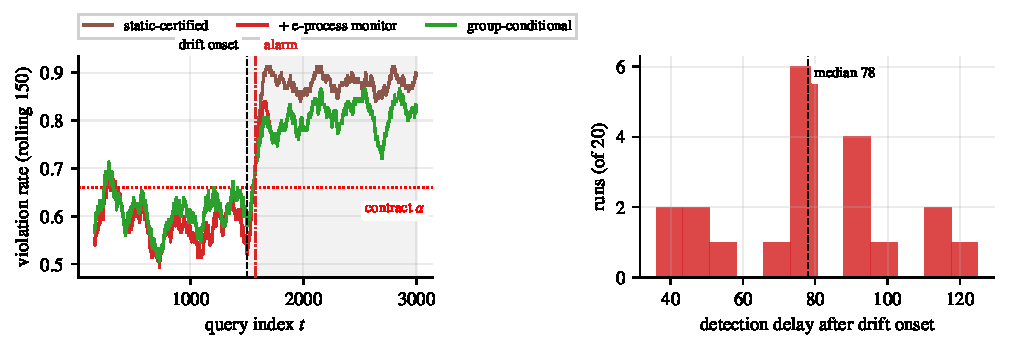
\includegraphics[width=0.85\textwidth]{figures/drift.pdf}
\caption{RQ4: workload drift on CRAG ($\alpha = 0.66$). Left: rolling
violation rate; the static certified policy breaks silently after the
shift at $t = 1500$; the e-process alarm (dash-dotted) triggers
recalibration. Right: detection delays over 20 seeded streams; no
false alarms on the 20 drift-free controls.}
\label{fig:drift}
\end{figure*}

\begin{figure}
\centering

\includegraphics[width=\columnwidth]{figures/drift2.pdf}
\caption{RQ4: measured detection delay (mean and p90 over 30 seeds per
drift magnitude) versus the Proposition~\ref{prop:delay} rate
$(\log(1/\delta) + \log(T|W|))/g^\ast$ --- mean delay sits below the
rate at every magnitude and the p90 tracks it within
0.6--1.0$\times$ (left). The $O(1)$ CUSUM recursion localizes the
changepoint to within a few queries for strong drifts (right). No
false alarms on the 200 drift-free controls.}
\label{fig:drift2}
\end{figure}

\paragraph{Workload drift}
A stream of 1500 static/slow queries followed by 1500 fast/real-time
queries (real losses, designed arrival order) breaks the marginally
certified policy: violation rises from 0.58 to 0.88 against a contract
of $\alpha = 0.66$, and without monitoring the system never knows
(Figure~\ref{fig:drift}). The e-process monitor fires at a median of 78
queries after onset (range 36--125 over 20 seeds) with no false
alarms across 20 drift-free control streams --- the expected
observation, since the per-stream Ville bound is $\delta/2 = .05$ and
a compliant stream's supermartingale in fact \emph{decays}, keeping
the realized false-alarm rate well below even that bound (confirmed
at finer resolution, $<1.5\%$, on the 200 control streams below).

\paragraph{Delay scaling and changepoint localization}
Varying the drift magnitude by mixing pools (post-change dynamic
fraction $\rho \in \{.5, .75, 1\}$, 30 seeds each) makes
Proposition~\ref{prop:delay} quantitatively checkable: for each
magnitude we compute the post-change optimal log-growth $g^\ast$ on the
monitor's bet grid ($.0071/.049/.137$) and compare measured delays
($760/203/82$ queries mean) against the rate
$(\log(1/\delta) + \log(T|W|))/g^\ast$. Mean delay sits below the rate
at every magnitude, is unaffected by the 1500-query compliant prefix,
and the rate is tight rather than ornamental: the p90 delay reaches
0.91--1.04$\times$ of it at moderate and strong drifts
(Figure~\ref{fig:drift2}). False alarms: none across the 200
drift-free control streams ($<1.5\%$ at 95\% confidence). The $O(1)$ recursion localizes the changepoint to a median
error of 4 queries at $\rho = 1$ and 10 queries at $\rho = .75$ ---
sharp enough that recalibration can discard exactly the pre-change
prefix.

\paragraph{Closed-loop certified recalibration}
Over 10 seeded streams we run the full loop: alarm $\to$ safe mode
(strongest rung --- a best-effort fallback that carries no certificate
on the unseen post-change distribution) for a 250-query labeled window
$\to$ fixed-sequence recertification on that window $\to$ deploy the
newly certified policy, which is where the post-drift guarantee
resides. The loop holds phase-2 violation to 0.819 versus 0.886
for the static policy, within half a point of the oracle that switches
to the post-change-certified policy at the exact drift time (0.815),
and beats a periodic reoptimizer that rechecks every 250 queries
(0.837) --- while spending less than the oracle (4.77 versus 4.94 mCNY
per query), because the certified post-alarm policy backs off from safe
mode as soon as the window certifies a cheaper ladder.

\paragraph{Multi-constraint monitoring with a global error budget}
Deployed contracts bind several dimensions, and an operator needs to
know \emph{which} constraint broke. We run four e-process monitors ---
correctness, hallucination, freshness, latency --- in parallel on the
certified CRAG policy, each at level $\delta_{\mathrm{mon}}/4$ so the
familywise false-alarm budget is a single global
$\delta_{\mathrm{mon}}$. Under a fresh-to-stale index transition, the
freshness monitor alarms after a median of 13.5 queries (range 5--25
over 20 seeds) while the correctness, hallucination, and latency
monitors --- whose constraints genuinely remain in contract ---
stay silent, and all four stay silent on 40 drift-free control
streams. The alarm is therefore also an \emph{attribution}: the
operator learns not just that the contract broke but that the index,
not the generator, is the failing knowledge source.

\paragraph{Lifetime operation across repeated alarms}
Proposition~\ref{prop:lifetime} prices an unbounded alarm--recalibrate
loop by geometric budget spending; we exercise it on a four-phase
stream (static $\to$ real-time $\to$ static $\to$ fast, 1200 queries
each, $\alpha = 0.85$, 20 seeds). Runs average 1.75 alarms; the first
drift is caught in a median of 98 queries and the second --- three
epochs later, on a quarter of the initial budget --- in 801, the
logarithmic delay price the proposition predicts. Recalibration
certifies a post-change policy in 84\% of alarm epochs; in the
remainder (the real-time phase, where even the strongest plan is out
of contract) the system correctly reports non-certifiability and
stays in flagged safe mode. Scheduled quiet-period rechecks recover
cheap policies after drifts revert: post-drift phases run at
violation 0.574 (static) against the contract while the
never-recalibrating baseline ranges from 0.603 up to complete failure
in the real-time phase, where every query it serves is out of
contract. No false alarms occurred
across 100 null streams ($<3\%$ at 95\% confidence) despite five
sequential tests per run --- the
geometric schedule keeps the lifetime promise it proves.

\paragraph{The price of knowing: audit accounting}
The monitor consumes audited violation indicators, which are not free:
on CRAG, exact-match short answers resolve 44\% of audits at
negligible cost, and the remaining 56\% need a judge call at 0.52 mCNY
--- an effective 0.29 mCNY per audited query, comparable to the
certified policy's own 0.30 mCNY deployment cost. Charging it
honestly: at 100\% audit the certified system's total cost of
ownership (deployment + audit + amortized calibration) is 0.60 mCNY
per query --- the ``20$\times$'' saving of Table~\ref{tab:main} is
10.0$\times$ once the meter includes the monitor. Auditing a random
25\% or 10\% of traffic restores the saving to 15.8$\times$ and
17.9$\times$ while keeping the guarantee intact on the audited
subsequence (Section~\ref{sec:monitor}): measured delays dilate almost
exactly as $1/r$ --- medians 74 / 343 / 878 queries at
$r = 1 / 0.25 / 0.1$, no false alarms at any rate --- so the audit
rate is a transparent dial between reaction time and monitoring spend.

\paragraph{Index staleness}
We re-execute the CRAG ladder under a 72-hour freshness contract in two
index states: in sync, and one week behind. When the index falls behind
\emph{silently}, the executor keeps serving dated web evidence that is
actually 168 hours older than it believes: per-rung joint
(correct-and-fresh) risk jumps from $(.79,.74,.71,.71)$ to
$(.94,.91,.91,.90)$ --- even the strongest plan now violates
$\alpha = 0.75$, so no amount of static escalation helps. The static
certified policy runs at phase-2 violation 0.926 and never knows; the
monitor alarms after a median of 117 queries (no false alarms on the
20 in-sync controls) and switches to the policy certified on stale-state
calibration data --- a freshness-honest re-execution whose filter
knows the lag, drops out-of-contract evidence, and escalates to the
still-fresh knowledge-graph API --- restoring violation to
$0.759 \approx \alpha$ at 2.52 mCNY per query, within 1\% of the
oracle that recalibrates exactly at the drift point. Freshness
contracts are thus operationally different from quality contracts:
staleness breaks every plan at once, and only detect-and-recertify ---
not conservative planning --- restores the guarantee.

\smallskip\noindent\textbf{Answer to RQ4:} \emph{drift is detected in
tens of queries with no false alarms and attributed to the failing
constraint, the measured delays match the proven bound at full and
subsampled audit rates, certified recalibration restores the contract
within 1\% of an oracle that knows the drift time, the geometric
budget schedule sustains repeated alarms over a full lifetime, and the
auditing that powers all of this costs at most half of the claimed
savings --- 10--18$\times$ instead of 20$\times$, reported honestly.}

\subsection{Answer to RQ5: generalization across LLM families and
serving backends}
\label{sec:exp-families}

\begin{table*}
\caption{RQ5: the same certified optimizer across four generator
families from four model developers, served via two backends --- three
commercial families hosted on one API platform (DashScope,
token-metered at each developer's list prices) and open-weight Gemma-3
served locally by Ollama, metered in GPU-seconds (HybridQA, quality
contract $\mathbf{1}[\text{F1}<0.5]$, $\delta = 0.1$; splits
300/500/600 over shared materialized retrieval). ``Viol.\ prob.'' is
the fraction of 200 repeated calibration/test draws whose exact
finite-population risk exceeds $\alpha$ (must be $\le \delta$);
``emp.'' is the empirical-no-certificate ablation; cells with no
violating draw report the one-sided 95\% binomial upper bound
$<.015$, the protocol's resolution at 200 draws, expected
under the certificate's built-in margin. On the noisier held-out
criterion the certified rates are 4.5\% (Qwen) and 9.5\% (DeepSeek),
still within $\delta$. At $\alpha = 0.35$
the Gemma-3 plan space is infeasible and \system\ reports
non-certifiability instead of deploying the least-bad plan.}
\label{tab:families}
\centering\scriptsize
\setlength{\tabcolsep}{2pt}
\begin{tabular*}{\tblwidth}{@{}l@{\extracolsep{\fill}}lcccccccccc@{}}
\toprule
& & & \multicolumn{2}{c}{Strongest fixed}
& \multicolumn{4}{c}{\system\ (certified)}
& \multicolumn{2}{c}{Utility router} & Oracle \\
\cmidrule(lr){4-5}\cmidrule(lr){6-9}\cmidrule(lr){10-11}
Family (serving) & $\alpha$ & metering
& risk & mCNY & risk & mCNY & saving & selected policy
& risk & mCNY & mCNY \\
\midrule
Qwen (DashScope)     & .35 & tokens & .300 & 7.29 & \textbf{.320} & 6.94 & 1.1$\times$ & ladder $q{=}.85$ & .395 & 0.37 & 3.18 \\
DeepSeek (DashScope) & .35 & tokens & .295 & 33.51 & \textbf{.337} & 2.02 & \textbf{16.6$\times$} & router $\lambda{=}32$ & .365 & 1.32 & 12.84 \\
GLM (DashScope)      & .35 & tokens & .277 & 22.71 & \textbf{.317} & 4.06 & 5.6$\times$ & router $\lambda{=}100$ & .355 & 3.76 & 13.68 \\
Gemma-3 (local Ollama) & .45 & GPU-s & .395 & 0.66 & \textbf{.432} & 0.57 & 1.2$\times$ & router $\lambda{=}178$ & .465 & 0.49 & 1.06 \\
\midrule
\multicolumn{3}{@{}l}{Viol.\ prob.\ over 200 draws (cert.\ / emp.)}
& \multicolumn{9}{l}{Qwen \textbf{$<$.015}/.300 \;\; DeepSeek
\textbf{$<$.015}/.095 \;\; GLM \textbf{$<$.015}/.055 \;\; Gemma-3
\textbf{$<$.015}/$<$.015 \;\; (pop.\ risk; $\delta{=}0.1$)} \\
\bottomrule
\end{tabular*}
\end{table*}

\begin{figure*}
\centering

\includegraphics[width=0.95\textwidth]{figures/families.pdf}
\caption{RQ5: the same certified optimizer across four generator
families (HybridQA, $\alpha = 0.35$; Gemma at $\alpha = 0.45$).
Retrieval is materialized once and shared; only the generator column
changes. Grey: the four fixed rungs; star: the certified policy. The
optimizer selects a different policy family per price structure and
stays below the contract line everywhere it certifies.}
\label{fig:families}
\end{figure*}

A fair objection to any cost-optimization result is that it may be an
artifact of one vendor's price sheet. We therefore hold the entire
framework fixed --- retrieval ladder, sufficiency scorers, candidate
families, certification --- and swap only the generator column across
four model families: Qwen \citep{qwen25}, DeepSeek
\citep{deepseekv3,deepseekr1}, GLM \citep{glm2024}, and open-weight
Gemma-3 \citep{gemma3} (Table~\ref{tab:families},
Figure~\ref{fig:families}). What this design varies is the model
developer and its price structure (four developers; two serving
backends: one hosted API platform and one local deployment); testing
robustness across independent hosting \emph{platforms} for the same
model would require replicating the ladder on a second API vendor,
which we leave outside scope and do not claim. Four results stand out.
(i) \emph{The guarantee transfers}: on every family where the contract
is feasible, over 200 repeated calibration/test draws per family the
certified policy's exact population risk never exceeds $\alpha$ in any
draw (below 1.5\% at 95\% confidence on all four families against the
$\delta = 0.1$
budget; up to 9.5\% on the noisier held-out criterion), while the
empirical-no-certificate ablation deploys truly out-of-contract
policies in up to 30\% of draws and the tuned utility router's single
deployment exceeds $\alpha$ on all four families. Uncertified selection
does not fail on one vendor's quirk; it fails everywhere. (ii) \emph{The
savings grow with the family's price spread}: certified cost drops
16.6$\times$ for DeepSeek and 5.6$\times$ for GLM against each family's
strongest plan, and the certified policy family itself changes with the
price structure --- a threshold ladder for Qwen's smooth tiering, jump
routers for DeepSeek and GLM, whose flash tiers are strong but whose
top tiers are disproportionately expensive. The optimizer discovers
this from data; nothing in the system encodes a vendor. (iii)
\emph{Infeasibility is reported, not hidden}: at $\alpha = 0.35$ no
Gemma-3 plan can meet the contract, and \system\ returns
non-certifiable instead of deploying the least-bad plan. (iv)
\emph{Cost-metric generality}: Gemma plans are metered in measured
GPU-seconds, and certification is indifferent to which currency the
cost column uses --- hosted token pricing and local GPU pricing flow
through the identical machinery.

\smallskip\noindent\textbf{Answer to RQ5:} \emph{the guarantee and the
savings are properties of the framework, not of a vendor: the
population-risk guarantee holds without a single violating draw on all
four families, savings reach 16.6$\times$ where price spreads are
wide, and the certified policy structure adapts to each family's
economics.}

\subsection{Answer to RQ6: knowledge-source selection and scalability}
\label{sec:exp-scale}

\paragraph{Acquisition-order selection}
On HybridQA we execute four physical plans for the table--text join at
a fixed flash-tier generator, so plan differences are purely
retrieval-side: \{table-first, text-first\} $\times$ \{lexical,
hybrid+rerank\}, with GPU-priced retrieval included in cost. Estimated
pool selectivity $\sigma$, computed from row-link cardinalities
\emph{before} execution, stratifies violation cleanly and monotonically
for every path: text-first-hybrid moves from 0.511 (lowest-$\sigma$
tercile) to 0.364 (highest), and the lexical paths pay a violation
premium over hybrid that grows with $\sigma$ --- the
selectivity-dependent crossover that source selection exploits. Feeding
the chooser family (fixed paths plus selectivity-threshold rules) to
the certification layer at $\alpha = 0.5$ certifies a mixed policy at
0.337 mCNY per query --- 31\% below the strongest fixed path (0.492)
with realized test violation $0.481 \le \alpha$. Everything a
relational optimizer does with selectivities --- pick the join order,
skip the expensive operator when the predicate is strong --- transfers
to knowledge acquisition, except that feasibility is established by the
test, not by the estimate.

\paragraph{Plan-space scalability and overhead}
Certification is a vectorized pass over the materialized execution
matrix, so enlarging the plan space is cheap: growing the threshold
grid from 69 to 97{,}365 candidates raises certification wall-clock to
8.5 s on HybridQA, 4.1 s on CRAG, and 0.9 s on ASQA --- still below the
cost of a single max-tier LLM call, with selection-proofness
(Theorem~\ref{thm:validity}) guaranteeing that the extra
$10^3\times$ candidates cost nothing in validity. The default
69-candidate space certifies in 5--8 ms; overall optimization overhead
is below $10^{-3}$ of a single LLM call, and the online policy adds one
score lookup per rung plus an $O(1)$ monitor update per query.
Materializing retrieval once and sharing it across the four generator
families of RQ5 removes three quarters of retrieval compute and
eliminates GPU contention between the reranker and locally served
generators. One caveat: more candidates are statistically free for
\emph{safety} but not automatically better for \emph{power} --- at
$n_{\mathrm{cal}} = 500$, a dense 8{,}029-candidate grid reaches the
contract boundary sooner on Qwen and certifies nothing, which is why
\system\ ships the compact curated space as the default.

\smallskip\noindent\textbf{Answer to RQ6:} \emph{selectivity-driven
source selection cuts retrieval-side cost 31\% under the same
certificate, and certification scales to $10^5$-candidate plan spaces
in seconds with provably unchanged validity.}
